% Grossmont College -- Chem 141 Lab 8: Propagation of Error
% Cameron Carroll
% May 2014


\documentclass[fleqn,titlepage]{article}

\renewcommand*\rmdefault{ppl}

\usepackage[version=3]{mhchem} % Package for chemical equation typesetting
\usepackage{tabu}
\usepackage{wasysym}
\usepackage{listings}
\usepackage{scrextend}
\lstset{language=Matlab}
\usepackage{multirow}

% set 1" margins on 8.5" x 11" paper
% top left is measured from 1", 1"
\topmargin 0in
\oddsidemargin 0in
\evensidemargin 0in
\headheight 0in
\headsep 0in
\topskip 0in
\textheight 9in
\textwidth 6.5in

\usepackage{graphicx} % Required for the inclusion of images

\setlength\parindent{0pt} % Removes all indentation from paragraphs

\renewcommand{\labelenumi}{\alph{enumi}.} % Make numbering in the enumerate environment by letter rather than number (e.g. section 6)

%\usepackage{times} % Uncomment to use the Times New Roman font

%----------------------------------------------------------------------------------------
% DOCUMENT INFORMATION
%----------------------------------------------------------------------------------------

\begin{document}

\begin{titlepage}
  \mbox{}\\[1.25cm]
  \textbf{\LARGE Cameron Carroll \\ Grossmont College}\\[2.25cm]
  \begin{center}
    \textbf{\huge Lab 7: \\ Propagation of Error}\\[2.50cm]
  \end{center}
  \textbf{\LARGE Professor: Martin Larter \\ Chemistry 141-0692} \\
  \vfill
  \center{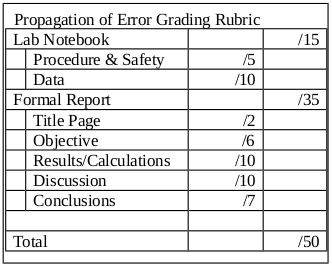
\includegraphics{./error_rubric}}
  \center{\textbf{\LARGE Performed --} {\LARGE March 20, 2014}}
  \center{\textbf{\LARGE Submitted --} {\LARGE May 27, 2014}}
\end{titlepage}

%----------------------------------------------------------------------------------------
% SECTION 1
%----------------------------------------------------------------------------------------
\section*{Objective}
  \paragraph{} This experiment explores how error propagates through calculations. We measured some simple physical data as precisely as possible and then used those values to demonstrate the techniques for error propagation.

%----------------------------------------------------------------------------------------
% SECTION 2
%----------------------------------------------------------------------------------------
\newpage
\section*{Discussion}
  \paragraph{} The first method, measuring with calipers to find the volume, yielded better accuracy with only 0.27\% deviation from the true value compared to measuring volume by displacement (at 7.05\% deviation.) This is expected, since the calipers have one more digit of uncertainty to its measurements than the graduated cylinders.
  \paragraph{} The precision turned out to be about the same using both methods, showing values to be within 0.0229 and 0.0225 $\frac{g}{cm^3}$ respectively according to the uncertainty propagation. 
  \paragraph{} I think it's worth noting, however, that the caliper method had a built-in precision loop before ever allowing a calculation. Due to the relative difficulty in actually operating this device, I only actually obtained these values after going to the professor and being told my precision is too low twice.
%----------------------------------------------------------------------------------------
% SECTION 3
%----------------------------------------------------------------------------------------
\section*{Conclusion}
My calculated densities were 2.928 and 2.729 $\frac{g}{cm^3}$ and their respective uncertainties were 0.0229 and 0.0225 $\frac{g}{cm^3}$. Also noteworthy is that the volume relative uncertainty term (7.8 and 8.25 $\cdot 10^3$) totally dominated the mass term (0.214 $\cdot 10^3$). This shows that even though that the instruments are more precise for the first method, thanks to the error propagation through the relatively complex calculation the density error comes out roughly the same.



\end{document}